\documentclass[10pt]{article}
\usepackage[OT1]{fontenc}
\usepackage[utf8]{inputenc}
\newtheorem{define}{Definition}
\usepackage{mathtools}
\newcommand{\R}{\mathbf{R}}
\newcommand{\transpose}{T}
\newcommand{\diag}{\operatorname{diag}}
\newcommand{\vol}{\operatorname{vol}}
\newcommand{\conv}{\operatorname{conv}}
\usepackage{tikz}
\usepackage{algorithm2e}
\usetikzlibrary{calc}
\usepackage{hyperref}
\usepackage[style=alphabetic, backend=biber]{biblatex}
\bibliography{refs.bib}

\oddsidemargin=0.15in
\evensidemargin=0.15in
\topmargin=-.5in
\textheight=9in
\textwidth=6.25in

\begin{document}
%--------------
%% preamble.tex
%% this should be included with a command like
%% %--------------
%% preamble.tex
%% this should be included with a command like
%% %--------------
%% preamble.tex
%% this should be included with a command like
%% \input{preamble.tex}
%% \lecture{1}{September 19, 2012 }{Aleksander Madry}{name of poor scribe}
% % Template based on Dan Spielman's template

\hbadness=10000
\vbadness=10000

\setlength{\oddsidemargin}{.25in}
\setlength{\evensidemargin}{.25in}
\setlength{\textwidth}{6in}
\setlength{\topmargin}{-0.4in}
\setlength{\textheight}{8.5in}


\newcommand{\handout}[5]{
   %\renewcommand{\thepage}{#1-\arabic{page}}
   \noindent
   \begin{center}
   \framebox{
      \vbox{
    \hbox to 5.78in { {\bf Topics in Theoretical Computer Science}
     	 \hfill #2 }
       \vspace{4mm}
       \hbox to 5.78in { {\Large \hfill #5  \hfill} }
       \vspace{2mm}
       \hbox to 5.78in { {\it #3 \hfill #4} }
      }
   }
   \end{center}
   \vspace*{4mm}
}

\newcommand{\lecture}[4]{\handout{#1}{#2}{Lecturer:
#3}{Scribes: #4}{Lecture #1}}
%% usage:
%% \lecture{1}{September 19, 2012 }{Aleksander Madry}{name of poor scribe}


\newtheorem{theorem}{Theorem}
\newtheorem{corollary}[theorem]{Corollary}
\newtheorem{lemma}[theorem]{Lemma}
\newtheorem{observation}[theorem]{Observation}
\newtheorem{proposition}[theorem]{Proposition}
\newtheorem{definition}[theorem]{Definition}
\newtheorem{claim}[theorem]{Claim}
\newtheorem{fact}[theorem]{Fact}
\newtheorem{assumption}[theorem]{Assumption}

\newcommand{\qed}{\rule{7pt}{7pt}}
\newcommand{\dis}{\mathop{\mbox{\rm d}}\nolimits}
\newcommand{\per}{\mathop{\mbox{\rm per}}\nolimits}
\newcommand{\area}{\mathop{\mbox{\rm area}}\nolimits}
\newcommand{\cw}{\mathop{\rm cw}\nolimits}
\newcommand{\ccw}{\mathop{\rm ccw}\nolimits}
\newcommand{\DIST}{\mathop{\mbox{\rm DIST}}\nolimits}
\newcommand{\OP}{\mathop{\mbox{\it OP}}\nolimits}
\newcommand{\OPprime}{\mathop{\mbox{\it OP}^{\,\prime}}\nolimits}
\newcommand{\ihat}{\hat{\imath}}
\newcommand{\jhat}{\hat{\jmath}}
\newcommand{\abs}[1]{\mathify{\left| #1 \right|}}

\newenvironment{proof}{\noindent{\bf Proof}\hspace*{1em}}{\qed\bigskip}
\newenvironment{proof-sketch}{\noindent{\bf Sketch of Proof}\hspace*{1em}}{\qed\bigskip}
\newenvironment{proof-idea}{\noindent{\bf Proof Idea}\hspace*{1em}}{\qed\bigskip}
\newenvironment{proof-of-lemma}[1]{\noindent{\bf Proof of Lemma #1}\hspace*{1em}}{\qed\bigskip}
\newenvironment{proof-attempt}{\noindent{\bf Proof Attempt}\hspace*{1em}}{\qed\bigskip}
\newenvironment{proofof}[1]{\noindent{\bf Proof}
of #1:\hspace*{1em}}{\qed\bigskip}
\newenvironment{remark}{\noindent{\bf Remark}\hspace*{1em}}{\bigskip}

% \makeatletter
% \@addtoreset{figure}{section}
% \@addtoreset{table}{section}
% \@addtoreset{equation}{section}
% \makeatother

\newcommand{\FOR}{{\bf for}}
\newcommand{\TO}{{\bf to}}
\newcommand{\DO}{{\bf do}}
\newcommand{\WHILE}{{\bf while}}
\newcommand{\AND}{{\bf and}}
\newcommand{\IF}{{\bf if}}
\newcommand{\THEN}{{\bf then}}
\newcommand{\ELSE}{{\bf else}}

% \renewcommand{\thefigure}{\thesection.\arabic{figure}}
% \renewcommand{\thetable}{\thesection.\arabic{table}}
% \renewcommand{\theequation}{\thesection.\arabic{equation}}

\makeatletter
\def\fnum@figure{{\bf Figure \thefigure}}
\def\fnum@table{{\bf Table \thetable}}
\long\def\@mycaption#1[#2]#3{\addcontentsline{\csname
  ext@#1\endcsname}{#1}{\protect\numberline{\csname 
  the#1\endcsname}{\ignorespaces #2}}\par
  \begingroup
    \@parboxrestore
    \small
    \@makecaption{\csname fnum@#1\endcsname}{\ignorespaces #3}\par
  \endgroup}
\def\mycaption{\refstepcounter\@captype \@dblarg{\@mycaption\@captype}}
\makeatother

\newcommand{\figcaption}[1]{\mycaption[]{#1}}
\newcommand{\tabcaption}[1]{\mycaption[]{#1}}
\newcommand{\head}[1]{\chapter[Lecture \##1]{}}
\newcommand{\mathify}[1]{\ifmmode{#1}\else\mbox{$#1$}\fi}
%\renewcommand{\Pr}[1]{\mathify{\mbox{Pr}\left[#1\right]}}
%\newcommand{\Exp}[1]{\mathify{\mbox{Exp}\left[#1\right]}}
\newcommand{\bigO}O
\newcommand{\set}[1]{\mathify{\left\{ #1 \right\}}}
\def\half{\frac{1}{2}}

\newcommand{\fig}[4]{
        \begin{figure}
        \setlength{\epsfysize}{#2}
        \vspace{3mm}
        \centerline{\epsfbox{#4}}
        \caption{#3} \label{#1}
        \end{figure}
        }

\newcommand{\ord}{{\rm ord}}

\providecommand{\norm}[1]{\lVert #1 \rVert}
\newcommand{\embed}{{\rm Embed}}
\newcommand{\qembed}{\mbox{$q$-Embed}}
\newcommand{\calh}{{\cal H}}
\newcommand{\lp}{{\rm LP}}

%% \lecture{1}{September 19, 2012 }{Aleksander Madry}{name of poor scribe}
% % Template based on Dan Spielman's template

\hbadness=10000
\vbadness=10000

\setlength{\oddsidemargin}{.25in}
\setlength{\evensidemargin}{.25in}
\setlength{\textwidth}{6in}
\setlength{\topmargin}{-0.4in}
\setlength{\textheight}{8.5in}


\newcommand{\handout}[5]{
   %\renewcommand{\thepage}{#1-\arabic{page}}
   \noindent
   \begin{center}
   \framebox{
      \vbox{
    \hbox to 5.78in { {\bf Topics in Theoretical Computer Science}
     	 \hfill #2 }
       \vspace{4mm}
       \hbox to 5.78in { {\Large \hfill #5  \hfill} }
       \vspace{2mm}
       \hbox to 5.78in { {\it #3 \hfill #4} }
      }
   }
   \end{center}
   \vspace*{4mm}
}

\newcommand{\lecture}[4]{\handout{#1}{#2}{Lecturer:
#3}{Scribes: #4}{Lecture #1}}
%% usage:
%% \lecture{1}{September 19, 2012 }{Aleksander Madry}{name of poor scribe}


\newtheorem{theorem}{Theorem}
\newtheorem{corollary}[theorem]{Corollary}
\newtheorem{lemma}[theorem]{Lemma}
\newtheorem{observation}[theorem]{Observation}
\newtheorem{proposition}[theorem]{Proposition}
\newtheorem{definition}[theorem]{Definition}
\newtheorem{claim}[theorem]{Claim}
\newtheorem{fact}[theorem]{Fact}
\newtheorem{assumption}[theorem]{Assumption}

\newcommand{\qed}{\rule{7pt}{7pt}}
\newcommand{\dis}{\mathop{\mbox{\rm d}}\nolimits}
\newcommand{\per}{\mathop{\mbox{\rm per}}\nolimits}
\newcommand{\area}{\mathop{\mbox{\rm area}}\nolimits}
\newcommand{\cw}{\mathop{\rm cw}\nolimits}
\newcommand{\ccw}{\mathop{\rm ccw}\nolimits}
\newcommand{\DIST}{\mathop{\mbox{\rm DIST}}\nolimits}
\newcommand{\OP}{\mathop{\mbox{\it OP}}\nolimits}
\newcommand{\OPprime}{\mathop{\mbox{\it OP}^{\,\prime}}\nolimits}
\newcommand{\ihat}{\hat{\imath}}
\newcommand{\jhat}{\hat{\jmath}}
\newcommand{\abs}[1]{\mathify{\left| #1 \right|}}

\newenvironment{proof}{\noindent{\bf Proof}\hspace*{1em}}{\qed\bigskip}
\newenvironment{proof-sketch}{\noindent{\bf Sketch of Proof}\hspace*{1em}}{\qed\bigskip}
\newenvironment{proof-idea}{\noindent{\bf Proof Idea}\hspace*{1em}}{\qed\bigskip}
\newenvironment{proof-of-lemma}[1]{\noindent{\bf Proof of Lemma #1}\hspace*{1em}}{\qed\bigskip}
\newenvironment{proof-attempt}{\noindent{\bf Proof Attempt}\hspace*{1em}}{\qed\bigskip}
\newenvironment{proofof}[1]{\noindent{\bf Proof}
of #1:\hspace*{1em}}{\qed\bigskip}
\newenvironment{remark}{\noindent{\bf Remark}\hspace*{1em}}{\bigskip}

% \makeatletter
% \@addtoreset{figure}{section}
% \@addtoreset{table}{section}
% \@addtoreset{equation}{section}
% \makeatother

\newcommand{\FOR}{{\bf for}}
\newcommand{\TO}{{\bf to}}
\newcommand{\DO}{{\bf do}}
\newcommand{\WHILE}{{\bf while}}
\newcommand{\AND}{{\bf and}}
\newcommand{\IF}{{\bf if}}
\newcommand{\THEN}{{\bf then}}
\newcommand{\ELSE}{{\bf else}}

% \renewcommand{\thefigure}{\thesection.\arabic{figure}}
% \renewcommand{\thetable}{\thesection.\arabic{table}}
% \renewcommand{\theequation}{\thesection.\arabic{equation}}

\makeatletter
\def\fnum@figure{{\bf Figure \thefigure}}
\def\fnum@table{{\bf Table \thetable}}
\long\def\@mycaption#1[#2]#3{\addcontentsline{\csname
  ext@#1\endcsname}{#1}{\protect\numberline{\csname 
  the#1\endcsname}{\ignorespaces #2}}\par
  \begingroup
    \@parboxrestore
    \small
    \@makecaption{\csname fnum@#1\endcsname}{\ignorespaces #3}\par
  \endgroup}
\def\mycaption{\refstepcounter\@captype \@dblarg{\@mycaption\@captype}}
\makeatother

\newcommand{\figcaption}[1]{\mycaption[]{#1}}
\newcommand{\tabcaption}[1]{\mycaption[]{#1}}
\newcommand{\head}[1]{\chapter[Lecture \##1]{}}
\newcommand{\mathify}[1]{\ifmmode{#1}\else\mbox{$#1$}\fi}
%\renewcommand{\Pr}[1]{\mathify{\mbox{Pr}\left[#1\right]}}
%\newcommand{\Exp}[1]{\mathify{\mbox{Exp}\left[#1\right]}}
\newcommand{\bigO}O
\newcommand{\set}[1]{\mathify{\left\{ #1 \right\}}}
\def\half{\frac{1}{2}}

\newcommand{\fig}[4]{
        \begin{figure}
        \setlength{\epsfysize}{#2}
        \vspace{3mm}
        \centerline{\epsfbox{#4}}
        \caption{#3} \label{#1}
        \end{figure}
        }

\newcommand{\ord}{{\rm ord}}

\providecommand{\norm}[1]{\lVert #1 \rVert}
\newcommand{\embed}{{\rm Embed}}
\newcommand{\qembed}{\mbox{$q$-Embed}}
\newcommand{\calh}{{\cal H}}
\newcommand{\lp}{{\rm LP}}

%% \lecture{1}{September 19, 2012 }{Aleksander Madry}{name of poor scribe}
% % Template based on Dan Spielman's template

\hbadness=10000
\vbadness=10000

\setlength{\oddsidemargin}{.25in}
\setlength{\evensidemargin}{.25in}
\setlength{\textwidth}{6in}
\setlength{\topmargin}{-0.4in}
\setlength{\textheight}{8.5in}


\newcommand{\handout}[5]{
   %\renewcommand{\thepage}{#1-\arabic{page}}
   \noindent
   \begin{center}
   \framebox{
      \vbox{
    \hbox to 5.78in { {\bf Topics in Theoretical Computer Science}
     	 \hfill #2 }
       \vspace{4mm}
       \hbox to 5.78in { {\Large \hfill #5  \hfill} }
       \vspace{2mm}
       \hbox to 5.78in { {\it #3 \hfill #4} }
      }
   }
   \end{center}
   \vspace*{4mm}
}

\newcommand{\lecture}[4]{\handout{#1}{#2}{Lecturer:
#3}{Scribes: #4}{Lecture #1}}
%% usage:
%% \lecture{1}{September 19, 2012 }{Aleksander Madry}{name of poor scribe}


\newtheorem{theorem}{Theorem}
\newtheorem{corollary}[theorem]{Corollary}
\newtheorem{lemma}[theorem]{Lemma}
\newtheorem{observation}[theorem]{Observation}
\newtheorem{proposition}[theorem]{Proposition}
\newtheorem{definition}[theorem]{Definition}
\newtheorem{claim}[theorem]{Claim}
\newtheorem{fact}[theorem]{Fact}
\newtheorem{assumption}[theorem]{Assumption}

\newcommand{\qed}{\rule{7pt}{7pt}}
\newcommand{\dis}{\mathop{\mbox{\rm d}}\nolimits}
\newcommand{\per}{\mathop{\mbox{\rm per}}\nolimits}
\newcommand{\area}{\mathop{\mbox{\rm area}}\nolimits}
\newcommand{\cw}{\mathop{\rm cw}\nolimits}
\newcommand{\ccw}{\mathop{\rm ccw}\nolimits}
\newcommand{\DIST}{\mathop{\mbox{\rm DIST}}\nolimits}
\newcommand{\OP}{\mathop{\mbox{\it OP}}\nolimits}
\newcommand{\OPprime}{\mathop{\mbox{\it OP}^{\,\prime}}\nolimits}
\newcommand{\ihat}{\hat{\imath}}
\newcommand{\jhat}{\hat{\jmath}}
\newcommand{\abs}[1]{\mathify{\left| #1 \right|}}

\newenvironment{proof}{\noindent{\bf Proof}\hspace*{1em}}{\qed\bigskip}
\newenvironment{proof-sketch}{\noindent{\bf Sketch of Proof}\hspace*{1em}}{\qed\bigskip}
\newenvironment{proof-idea}{\noindent{\bf Proof Idea}\hspace*{1em}}{\qed\bigskip}
\newenvironment{proof-of-lemma}[1]{\noindent{\bf Proof of Lemma #1}\hspace*{1em}}{\qed\bigskip}
\newenvironment{proof-attempt}{\noindent{\bf Proof Attempt}\hspace*{1em}}{\qed\bigskip}
\newenvironment{proofof}[1]{\noindent{\bf Proof}
of #1:\hspace*{1em}}{\qed\bigskip}
\newenvironment{remark}{\noindent{\bf Remark}\hspace*{1em}}{\bigskip}

% \makeatletter
% \@addtoreset{figure}{section}
% \@addtoreset{table}{section}
% \@addtoreset{equation}{section}
% \makeatother

\newcommand{\FOR}{{\bf for}}
\newcommand{\TO}{{\bf to}}
\newcommand{\DO}{{\bf do}}
\newcommand{\WHILE}{{\bf while}}
\newcommand{\AND}{{\bf and}}
\newcommand{\IF}{{\bf if}}
\newcommand{\THEN}{{\bf then}}
\newcommand{\ELSE}{{\bf else}}

% \renewcommand{\thefigure}{\thesection.\arabic{figure}}
% \renewcommand{\thetable}{\thesection.\arabic{table}}
% \renewcommand{\theequation}{\thesection.\arabic{equation}}

\makeatletter
\def\fnum@figure{{\bf Figure \thefigure}}
\def\fnum@table{{\bf Table \thetable}}
\long\def\@mycaption#1[#2]#3{\addcontentsline{\csname
  ext@#1\endcsname}{#1}{\protect\numberline{\csname 
  the#1\endcsname}{\ignorespaces #2}}\par
  \begingroup
    \@parboxrestore
    \small
    \@makecaption{\csname fnum@#1\endcsname}{\ignorespaces #3}\par
  \endgroup}
\def\mycaption{\refstepcounter\@captype \@dblarg{\@mycaption\@captype}}
\makeatother

\newcommand{\figcaption}[1]{\mycaption[]{#1}}
\newcommand{\tabcaption}[1]{\mycaption[]{#1}}
\newcommand{\head}[1]{\chapter[Lecture \##1]{}}
\newcommand{\mathify}[1]{\ifmmode{#1}\else\mbox{$#1$}\fi}
%\renewcommand{\Pr}[1]{\mathify{\mbox{Pr}\left[#1\right]}}
%\newcommand{\Exp}[1]{\mathify{\mbox{Exp}\left[#1\right]}}
\newcommand{\bigO}O
\newcommand{\set}[1]{\mathify{\left\{ #1 \right\}}}
\def\half{\frac{1}{2}}

\newcommand{\fig}[4]{
        \begin{figure}
        \setlength{\epsfysize}{#2}
        \vspace{3mm}
        \centerline{\epsfbox{#4}}
        \caption{#3} \label{#1}
        \end{figure}
        }

\newcommand{\ord}{{\rm ord}}

\providecommand{\norm}[1]{\lVert #1 \rVert}
\newcommand{\embed}{{\rm Embed}}
\newcommand{\qembed}{\mbox{$q$-Embed}}
\newcommand{\calh}{{\cal H}}
\newcommand{\lp}{{\rm LP}}

\lecture{11}{April 27, 2015}{Ola Svensson}{Louis Faucon, Andreas Haupt}

\section{Introduction}
In today's lecture, the \emph{Ellipsoid Method} is introduced, which has been the first weakly polynomial-time\footnote{An algorithm is weakly polynomial if its running time not only depends on the number of inputs, but also logarithmically on their size.} algorithm for Linear Programming. The method was originally proposed in \cite{shor77} in the more general context of convex optimization problems. \cite{khachiyan79} applied this to Linear Programming. The method is fast in theory, but very slow in practice as experiments show. A major advantage of the Ellipsoid method is that it can solve even exponentially-sized LPs for which an efficient so-called separation oracle exists. This is the case i.e. for the Traveling Salesperson problem, as we see in \autoref{subsec:seporacle}. Another widely used solution method for LPs, the \emph{Interior Point Method} introduced by \cite{karmarkar89}, will not be covered here, as it does not have this advantage, although it is proved efficient in theory and seems to be competitive in practice. 
\subsection{Motivation}\label{sec:motivation}
Suppose\footnote{This motivation is due to \protect\cite{lovaszschrijver}}, you are lion hunter in Sahara and there is at least one lion in it. If you have plenty of time, you could catch one lion by building a fence that splits Sahara into two pieces, to look on which side of the fence the lion is, building a fence that splits this part of Sahara in two parts, etc. When the area of the piece of Sahara we know the lion is in is smaller than any lion can be, we have caught it. The success of this strategy and the time needed to catch the lion depend on the following:
\begin{itemize}
\item How big is Sahara?
\item When to terminate, i.e.: How small is the smallest lion?
\end{itemize}
Now we make the transfer to the problem we intend to solve:
\subsection{Problem Statement}
We would like to find, given a convex set $P\subseteq \R^n$, an $x \in P$ or decide, that $P = \emptyset$.

If we can solve this problem efficiently, we can also solve an arbitrary LP efficiently, using the following: We consider the primal-dual polytope, i.e. the LP that contains all the inequalities and equalities of the dual and the primal LP and the equality of values. This means for the LP $\max_{Ax\le b} c^\transpose x$ the polytope
\[
\{x \in \R^n |Ax \le b, yA=c, y \ge 0, yb=cx\}.
\]
Suppose, there are $k$ inequalities. At first, we test, whether the primal-dual polytope is feasible; if not, there is no optimal solution to the LP by the duality theorem. Otherwise, we test, whether the LP becomes infeasible if we substitute for one of the inequalities equality. If this makes the LP infeasible, that means, no feasible solution of the primal-dual takes the substituted inequality with equality, hence it is redundant and can be deleted. If the LP remains feasible that way, we make the substitution having now an LP with less inequalities. Iteratively, we obtain a maximization subject to a number of equality constraints. This can be solved with Gaussian Elimination and yields an optimal solution in a polynomial number of feasibility oracle calls and polynomial time. In the next section, we describe the Ellipsoid Method that solves the feasibility problem and present related geometric propositions.
\section{The Ellipsoid Algorithm}
The Feasibility Problem is solved by \autoref{algo:ellips} if this algorithm terminates. Its idea is to 
\begin{algorithm}
\caption[a]{Ellipsoid Method}
\KwIn{Convex Set $P$, $\varepsilon > 0$ such that $\vol (P) \ge \varepsilon$}
\KwOut{Feasibility of $P$}
Start with an Ellipsoid $E_0 \supseteq P$\;
\While{center of $a_k$ of $E_k$ not in $P$ or $\vol (E_k) < \varepsilon$}{Let $c \in \R^n$, such that $\{x \in \R^n | c^\transpose x < c^\transpose a_k \} \supseteq P$ i.e. pick a hyperplane that \emph{separates} $P$\;
Let $E_{k+1}$ be the smallest ellipsoid, such that $E_{k+1} \supseteq E_k \cap \{x \in \R^n | c^\transpose x < c^\transpose a_k\}$\;
$k \leftarrow k+1$\;}
\eIf{center of $E_k$ in $P$}{\Return Yes\;}{\Return No\;}
\label{algo:ellips}
\end{algorithm}
\autoref{fig:ellipsoidex}
\begin{figure}[ht]
  \centering
  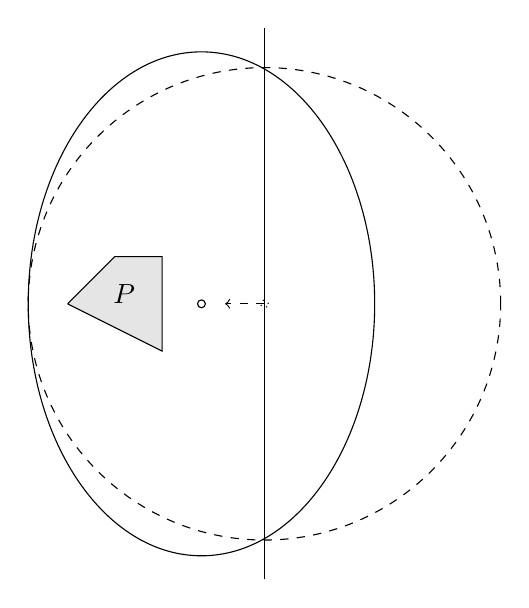
\begin{tikzpicture}
    \begin{scope}[scale=0.6]
      \draw[fill=gray!20!white] (0,0) -- (1,1) -- (2,1) -- (2,-1) -- (0,0);
      \node at (1.2,0.2) {$P$};
    \end{scope}
    \draw[dashed] (2.5,0) ellipse (3cm and 3cm);
    \draw[dotted] (2.5, 0) circle (0.05);
    \draw[] (2.5, -3.5) -- (2.5, 3.5);
    \draw[dashed] (2.5, 0) edge[->] (2, 0);
    \draw[] (1.7, 0) ellipse (2.2cm and 3.2cm);
    \draw[] (1.7, 0) circle (0.05);
  \end{tikzpicture}
  \caption{One step of the Ellipsoid method: Starting with the dashed ellipsoid we obtain the smaller ellipsoid (using a separating hyperplane).}
  \label{fig:ellipsoidex}
\end{figure}
We review some properties of ellipsoids.
\subsection{Ellipsoids}
Recall that $A \in \R^{n \times n}$ is called positive definite, iff it is symmetric, i.e. $A = A^\transpose$ and 
\[
\forall x \in \R^n\setminus \{0\} \colon x^\transpose A x > 0
\]
i.e. that the scalar product induced by $A$ is positive definite. This class of matrices is closed under inversion and for any positive definite matrix $A$ there exists a matrix $A^{\frac{1}{2}}$, such that
\[
A = A^{\frac{1}{2}} (A^{\frac{1}{2}})^\transpose.
\]
\begin{definition}[Ellipsoid]
An ellipsoid $E(a,A)$ with center $a \in \R^n$ and positive definite matrix $A$ is defined as
\[
E(a,A) \coloneqq \{x \in \R^n | (x-a)^{\transpose} A^{-1} (x-a) \le 1 \} = \{x \in \R^n | \| (A^{-1})^\frac{1}{2} (x-a) \| \le 1 \}
\]
\end{definition}
In fact, $E(a,A)$ is just the image of the unit ball $\{x\in \R^n | \|x\|\le 1\}$ under the affine-linear map $x \mapsto A^{\frac{1}{2}} x + a$. As an example, consider $E(a,A)$ with 
\begin{align}
A^{\frac{1}{2}} &= \begin{pmatrix} 2 & 0 \\ 0 & 1 \end{pmatrix} & a &= \begin{pmatrix} 4 \\ 0 \end{pmatrix}. \label{eq:ellipsoidexample}
\end{align}
The result is \autoref{fig:ellipsoidexample}. We now would like to come closer 
\begin{figure}
\centering
\begin{tikzpicture}[scale=2]
\begin{scope}
    \draw[->] (-1.1,0) -- (6.1,0) node[right] {$x$} coordinate(x axis);
    \draw[->] (0,-1.1) -- (0,1.1) node[above] {$y$} coordinate(y axis);
    \foreach \x/\xtext in {-1,0,...,6}
      \draw[xshift=\x cm] (0pt,1pt) -- (0pt,-1pt) node[below,fill=white] {$\xtext$};
    \foreach \y/\ytext in {-1, -.5/-\frac{1}{2}, .5/\frac{1}{2}, 1}
      \draw[yshift=\y cm] (1pt,0pt) -- (-1pt,0pt) node[left,fill=white] {$\ytext$};
  \end{scope}
\draw (0,0) circle (1cm);
\draw (4,0) ellipse (2cm and 1cm);
\path (.4,1) edge [bend left, ->] node[above]{$x \mapsto \begin{pmatrix} 2 & 0 \\ 0 & 1 \end{pmatrix} x +  \begin{pmatrix} 4 \\ 0 \end{pmatrix}$} (3.4,1);
\end{tikzpicture}
\caption{On the left the unit ball in $\R^2$, the affine map mapping the unit circle to the ellipsoid from \protect\autoref{eq:ellipsoidexample}.}
\label{fig:ellipsoidexample}
\end{figure}
\begin{lemma}[Half-Ball Lemma]\label{lem:halfball}
The half-ball
\[
H = \{x \in \R^n | \| x \| \le 1, x_1 \ge 0 \}
\]
is contained in the ellipsoid
\[
E = \left\{ x \in \R^n \middle| \left(\frac{n+1}{n}\right)^2\left(x_1 - \frac{1}{n+1}\right)^2 + \frac{n^2-1}{n^2} \sum_{i=2}^n x_i^2 \le 1 \right\}
\]
\end{lemma}
\begin{proof}
Let $x$ be in the half-ball, we have $\sum_{i=1}^n x_i^2 \le 1, x_1 \ge 0$, then one calculates :
\begin{align*}
\left(\frac{n+1}{n} \right)^2 \left(x_1-\frac{1}{n+1}\right)^2 + \frac{n^2-1}{n^2} \sum_{i=2}^n x_i^2 
&\leq \left(\frac{n+1}{n} \right)^2 \left(x_1-\frac{1}{n+1}\right)^2 + \frac{n^2-1}{n^2}(1 - x_1^2)\\
&\leq \frac{2(n+1)}{n^2} x_1^2-\frac{2(n+1)}{n^2}x_1 + 1\\
&\leq 1 
\end{align*}
as  $0 \leq x_1 \leq 1$
\end{proof}
We remark, that this ellipsoid is $E(a,A)$ with
\begin{align*}
a &= \frac{1}{n+1} e_1 &  A^{\frac{1}{2}}&= \diag \left(\frac{n}{n+1}, \frac{n}{\sqrt{n^2-1}}, \dots, \frac{n}{\sqrt{n^2-1}}\right),
\end{align*}
where $e_1$ is the first canonical basis vector and $\diag (x_1, \dots, x_n)$ denotes the matrix with $x_1, \dots, x_n$ on its diagonal. In dimension two, this ellipsoid is given by \autoref{fig:halfball}.
\begin{figure}
\centering
\begin{tikzpicture}[scale=2]
\begin{scope}
    \draw[->] (-1.6,0) -- (1.6,0) node[right] {$x$} coordinate(x axis);
    \draw[->] (0,-1.1) -- (0,1.1) node[above] {$y$} coordinate(y axis);
    \foreach \x/\xtext in {-1,0,...,1}
      \draw[xshift=\x cm] (0pt,1pt) -- (0pt,-1pt) node[below,fill=white] {$\xtext$};
    \foreach \y/\ytext in {-1, -.5/-\frac{1}{2}, .5/\frac{1}{2}, 1}
      \draw[yshift=\y cm] (1pt,0pt) -- (-1pt,0pt) node[left,fill=white] {$\ytext$};
  \end{scope}
\draw (1,0) arc (0:180:1cm);
\draw (0,0.33333) ellipse (1.15 and 0.6666);
\end{tikzpicture}
\caption{The smallest ellipsoid containing the half-ball in dimension two}
\label{fig:halfball}
\end{figure}
What is the volume of our ellipsoid? For sure, the translation by $a$ does not matter for the volume. The change of volume is thus given by $\det (A^{\frac{1}{2}})$ and we have
\[
\det (A^{\frac{1}{2}}) = \frac{n}{n+1} (\frac{n}{\sqrt{n^2-1}})^{n-1} \le e^{-\frac{1}{n+1}} (e^{\frac{1}{n^2-1}})^{\frac{n-1}{2}} = e^{-\frac{1}{2(n+1)}}
\]
using $e^x \geq 1 + x$.
\begin{corollary}
If $E_n$ denotes the unit ball in $n$ dimensions, and $E$ the corresponding ellipsoid from Lemma \ref{lem:halfball}, then
\[
\frac{\vol (E)}{\vol (E_n)} = \det (A^{\frac{1}{2}}) \le e^{-\frac{1}{2(n+1)}}<1
\]
\end{corollary}
More generally, we may consider the half-ball in any direction $d$. Then the ellipsoid becomes $E = (-\frac{d}{n+1}, F)$, where $F = \frac{n^2}{n^2-1} (I - \frac{2}{n+1} dd^\transpose)$ and $I$ denotes the identity matrix. Now, given $E_k = (a_k, A_k)$ and some hyperplane which goes through $a_k$, we can apply the inverse transformation $x \mapsto (A^{-1})^{\frac{1}{2}} (x-a)$ of the transformation that mapped the unit ball to our polytope. One observes, that
\begin{itemize}
\item $E_k$ becomes the unit ball. 
\item The hyperplane now cuts the unit ball in half-balls $\{x\in \R^n | c^\transpose x \le c^\transpose a_k \} \xmapsto{T^{-1}} \{y\in \R^n | c^\transpose (A^{\frac{1}{2}} y + a_k ) \le c^\transpose a_k\} = \{y \in \R^n | (c^\transpose A^{\frac{1}{2}}) y \le 0 \}$
\end{itemize}
Finally applying again the transformation to the ellipsoid given by Lemma \ref{lem:halfball} gives us the desired ellipsoid.

The next section is concerned with further technical aspects of the Ellipsoid Method.
\section{Initial Ellipsoid, Stopping and Minimal Polytope Size}
We now discuss three remaining questions for the special case of 0-1 LPs i.e. LPs whose polytope $P$ is of the form $P = \conv (S), S \subseteq \{0,1\}^n$. We furthermore assume them to be full-dimensional. For the initial ellipsoid, $E_0 \coloneqq E(a,\sqrt{n}E_n)$, $a=(\frac{1}{2}, \dots, \frac{1}{2})$ is an obvious choice. The minimum size of a polytope and a stopping criterion are discussed in the subsections below.
\subsection{Minimum Size of a Polytope}
Let $v_0 \in P$. Since $P$ is full-dimensional, there exist $v_1, \dots, v_n \in P$, whose convex hull forms a simplex. It has volume
\[
\frac{1}{n!} \left\lvert\det ((v_0-v_1, \dots, v_0-v_n))\right\rvert
\]
Therefore, $\vol (P) \ge \frac{1}{n!}$ (as all entries in the vectors are integral).
\subsection{Stopping Criterion}
We observe, that the initial ellipsoid has a volume of at most $\sqrt{n}^{n} 2^n$, which means that $\log (\vol (E_0)) = O(n \log n)$. We can stop the algorithm if $\vol (E_k) < \vol(P)$. Furthermore, we have
\[
\vol (E_k)\le e^{-\frac{k}{2(n+1)}} \vol (E_0)
\]
This yields, that after at most $O(n \log (\frac{\vol (E_0)}{\vol (P)}))$ iterations the algorithm terminates.
\section{Separation Oracles}\label{sec:oracles}
The running time of the Ellipsoid Method is independent of the number of constraints. To solve the feasibility problem for a convex $P$ with the Ellipsoid Method, you only need to design a separation oracle that decides, given a point $x^*$, whether $x^*\in P$ and if not outputs $a \in \R^n, b \in \R$, such that $a^\transpose x \le b, \forall x \in P$ and $a^\transpose x^* > b$. Although the argument from the introduction cannot be made in this case, the method can still be used to solve LPs as is proved in \cite{consequences}. In a last part, we show, that for the Travelling Salesperson Problem, an efficient algorithm exists.
\subsection{Separation Oracle for Travelling Salesperson Problem}\label{subsec:seporacle}
The Travelling Salesperson Problem asks for a minimum length Hamiltonian circuit in an undirected weighted graph $G$. For $x_e \in \{0,1\}^{E(G)}$ we let $x_e$ be the incidence vector of a tour. A popular LP relaxation for this problem is
\begin{align}
\min \sum_{e \in E(G)} &d(e) x_e\nonumber \\
\sum_{e \in \delta (v)}& x_e =2 , \forall v \in V(G) \label{eq:cutinequalities}\\
\sum_{e \in \delta(S)} &x_e \ge 2 , \forall S \subseteq V\nonumber\\
 &x \ge 0\nonumber
\end{align}
This LP can be solved efficiently using the Ellipsoid method. The inequalities \autoref{eq:cutinequalities} can be efficiently separated by calculating the minimum $s$-$t$-cut for all $s,t \in V$, which yields a polynomial separation oracle.


\printbibliography

\end{document}